\chapter{Implementation internals}
\addtocontents{toc}{\protect\setcounter{tocdepth}{0}}
This section provides insights on the code from a programmer's point of view. We will not focus on algorithms here, as we already did that in \cref{chaptImplementation}. The main focus here is on data representation and division of code into multiple modules.

\section{Data representation}
As a result of using multiple libraries for a multitude of tasks, we have to deal with a lot of different data representations of the same objects. 

We will introduce the data structures that are used to represent one in-game object for multiple purposes. We can see how different data types are converted in~\cref{fig:conversions}.

\begin{figure}
        \centering
        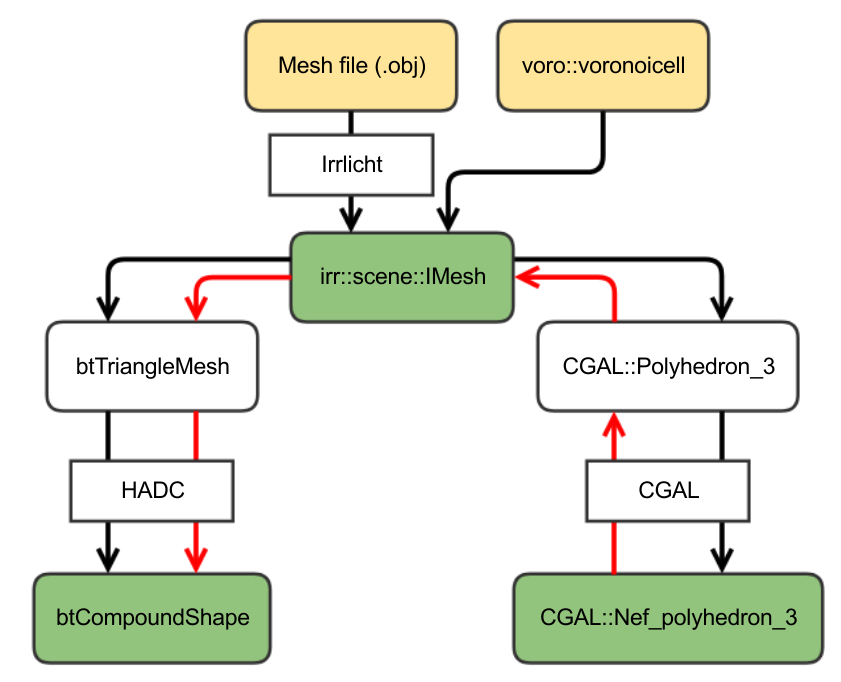
\includegraphics[width=\textwidth]{img/conversions}
        \caption{Data conversion diagram. Input formats - yellow, required formats - green. Black lines show used conversions, red lines show required process after a change of the shape of an object. Rectangles signify the library used to make the conversion, if none a member function of {\tt gg::MMeshManipulators} is used.}
        \label{fig:conversions}
\end{figure}

\subsection*{\tt btRigidBody}
\emph{Bullet physics} uses this class to hold information about a rigid collision object. For us, most important part of the body is a collision shape. \todo{je nekde napsany ze (a jak a proc) pouzivas bullet (a irrlicht)?}

The collision shape can be of multiple types, most notably a convex hull or a primitive geometric shape, a triangular mesh or a compound shape. We need the collision shape to be as close to a visual mesh as possible. Because calculating collision between triangular meshes is not implemented in the \emph{Bullet physics} and would be too costly\todo{even if implemented}, we choose the representation by compound shape..

One more parameter of {\tt btRigidBody} to consider is the object mass. Bodies with mass set to zero (or negative value) are considered static objects and do not move. Bodies with positive mass react to gravity and other external forces, their centre of gravity is set to their respective origin of local coordinates. This poses a problem when the origin is not inside the object. Our solution is to manually translate the mesh to the origin. \todo{ref link do kodu kde to delas}

\subsection*{\tt irr::scene::ISceneNode} 
Graphical object in the \emph{Irrlicht engine} is represented by this class. It is an abstract class instantiated into multiple types of graphical objects, \eg lights, cameras, animations, particle systems. We are using {\tt irr::scene::IMeshSceneNode} for our objects. The mesh information in {\tt irr::scene::IMeshSceneNode} is stored in {\tt irr::scene::IMesh}. 

\subsection*{\tt irr::scene::IMesh} 
This class stores the mesh information in multiple mesh buffers. Each buffer has an array of vertices and an array of indices. Every index in the array of indices refers to one vertex. However, we found out that not every vertex is referred to, and therefore valid. Indices divided into consecutive non-intersecting triples form a triangular face of a mesh. 

The fact that the mesh is split into multiple mesh buffers and that every face in each mesh buffer must be complete needs to be addressed when converting the data \todo{converting from what?}. If two neighbouring faces are both stored in a different mesh buffer, their common edge is \todo{must be?} stored twice. When converting to {\tt CGAL::Nef\_polyhedron\_3}, the duplicity in edges bans us from copying the mesh face by face and requires filtering, because overlapping geometry is not allowed in {\tt CGAL::Nef\_polyhedron\_3}. \todo{tuhle vetu je potreba rozepsat: 1. je to prima kolize s pozadavkama nef polyhedronama z CGAL, 2. overlapping geometry tam totiz pusobi potize, 3. co to znamena (nemuzeme to zkopirovat fejs2fejs 4. jak to resime (co presne se vyfiltruje)}

\subsection*{\tt CGAL::Nef\_polyhedron\_3}
\todo {text here}

\subsection*{\tt gg::MObject} 
{\tt gg::MObject} is a class designed to unite all data about one in-game object into one structure. It includes {\tt irr::scene::ISceneNode}, {\tt CGAL::Nef\_polyhedron\_3} and {\tt btRigidBody}. It implements the mechanism ensuring that upon deletion of an object, its parts are first removed from their respective engines, and then safely deallocated before {\tt gg::MObject} itself is destroyed.



\section{Modules}
In this section, we describe the functionality of each program module. Third party software is not be described here, details about used libraries can be found in \cref{chapt:technology}. Interactions between modules are visualised in \cref{fig:modules}. \emph{Irrlicht Engine} is not present in the diagram because we do not structurally depend on it. Every module is contained in a file of the same name, as a class with that name prefixed with letter M (\ie Object Creator can be found in file ObjectCreator.cpp and is implemented as class {\tt gg::MObjectCreator}). Also, namespace {\tt gg} identifies exact components of the application implemented for this thesis.

\begin{figure}
        \centering
        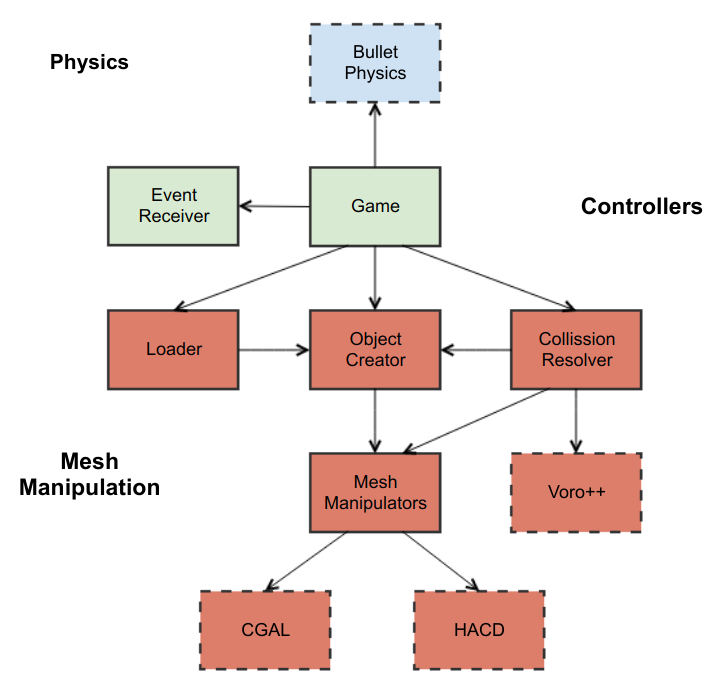
\includegraphics[width=\textwidth]{img/objectmodel}
        \caption{Software architecture shown on diagram of relationships of program modules. Third party software is highlighted in dashed rectangles.}
        \label{fig:modules}
\end{figure}

\subsection*{Game}
\todo{Chyba --- pouzivat nadpis jako soucast textu (na kterou se navic odkazujes) nejde, stylisticky text musi bejt kompletni i bez nadpisu. Nadpisy ber jen jako labely na ktery lidi delaj lidsky GOTO. Udelej z toho seznam, ty subsectiony jsou stejne moc kratky. Pokud k nejaky chces napsat vic (object creator) tak nejdriv hod seznam a pak dej subsection ktera popisuje fungovani ObjectCreatoru.}
This module holds {\tt gg::MGame} class which is the core of the application. The communication with the physics engine,  the graphical engine and mesh manipulation parts of the software is managed from here.

\subsection*{Event Receiver}
This class\todo{class nebo module?} is an implementation of {\tt irr::IEventReceiver} from Irrlicht engine and it is used to read the user input.

\subsection*{Loader}
The Loader is only used for initializing the application. It parses the data that describe the game environment from the given file\todo{all data in 1 file?}, constructs the objects using {\tt gg::MObjectCreator}, and returns the set of constructed objects.

\subsection*{Object Creator}
We use this class as a Builder pattern in order to initialize the data contained inside {\tt gg::MObject}, namely {\tt btRigidBody, CGAL::Nef\_polyhedron\_3} and {\tt irr::scene::ISceneNode}.

There are three member functions that allow us to create {\tt gg::MObject}s  with different behaviours from the same set of input parameters (see \cref{sec:data}). We can create a destructible object, an indestructible object with box collision shape and a rectangular indestructible object without input mesh. Those functions are exclusively used at initialization, as they generate a new set \todo{tohle neni duvod proc by mely bejt pouzivany jen pri initu.} of member variables, and their parameters come in a text form.

Two more kinds of objects can be created a projectile that \todo{asi chybi dvojtecka?} is shot from the given position with the given impulse and a destructible object with temporary collision shape (sphere shaped). Because the object with temporary collision shape is constructed while the game is being played and construction of {\tt CGAL::Nef\_polyhedron\_3} can take a longer time, it requires to have the {\tt CGAL::Nef\_polyhedron\_3} given in parameter\todo{hra je hrana \& a vyroba NEF trva dlouho $\implies$ NEF je potreba na vyrobu temporary objectu? nedava moc smysl.}. Indestructible objects do not require {\tt CGAL::Nef\_polyhedron\_3} and therefore the shooting is not limited by their construction time\todo{tohle asi ani nezminuj, 1. strela neni indestructible (jen ji tu destrukcu nesimulujes) 2. jeste aby vyrobeni obycejny nesimulovany strely neco trvalo! :D}.

\subsection*{Collision Resolver}
After every collision, Collision Resolver decides what to do with it, and in the case of destruction, takes care of the whole process\todo{tohle je hodne utrzkovity...}. To process the collision, {\tt gg::MCollisionResolver} owns both Mesh subtraction and Convex Decomposition threads\todo{Tu kolizi vyresi jen tim ze vlastni obe ty vlakna?}. The Voronoi cell generation is also done in this module\todo{Asi by bylo lepsi celej ten proces rozepsat, nebo se odkazat na nejakej kompletni popis jinde}. Collision resolver heavily relies upon Mesh Manipulators utility functions because many data conversions are happening in here.\todo{Tuhle vetu obratit: Conversions between data formats that are required during the process are externalized to Mesh Manipulators module to maintain the code readable?}

\subsection*{Mesh Manipulators}
Mesh Manipulators provides set of public static \todo{je k necemu dobry ze jsou public static? jestli ne tak bych to uplne vynechal a napsal jen ze to je hlavne ke konverzi tech reprezentaci.} functions. Because different libraries are used for physics simulation, rendering and geometric manipulation, those functions provide means for converting data between different formats.
